\section{Sprint 4} 

Il progetto di riferimento per questo sprint è it.unibo.ddrSystem5.

\textbf{OBIETTIVO}: creazione di un sistema con un robot che, data una stanza con ostacoli (sia muri sia valigie), la esplori in maniera autonoma e ne costruisca una mappa. Sulla mappa dovranno essere evidenziati tutti gli ostacoli individuati. 

\subsection{Work Plan}
\begin{enumerate}
\item definizione di valigia come nuova entità del sistema;
\item definizione di "fine esplorazione" di una stanza con ostacoli fissi (muri e valigie);
\item creazione di una strategia per la gestione degli ostacoli;
\item creazione di una strategia per terminare l'esplorazione di una stanza con ostacoli.
\end{enumerate}

\subsection{Analisi dei requisiti}

\textbf{Che cosa si intende per valigia?}\\
La valigia rappresenta un ostacolo fisso disposto all'interno della stanza. Essa può trovarsi in mezzo alla stanza oppure adiacente ad 1 o 2 pareti. Una valigia è un ostacolo che può essere aggirato dal robot, quindi non sarà possibile per il robot esplorare la cella occupata della valigia, ma solo le celle adiacenti.
Nel caso in cui un ostacolo si trovi parzialmente su una cella, essa viene comunque considerata dal robot interamente occupata da un ostacolo.
Inoltre, in questo sistema non si tiene conto della differenza tra un muro ed una fila lunga di valigie: entrambi determinano il confine della stanza. Perciò, in presenza di un ostacolo, se il robot riesce a raggiungere con un altro percorso il proprio obiettivo, allora continuerà l'esplorazione, in caso negativo significherà che il robot ha individuato i confini.


\textbf{Che cosa si intende per "fine esplorazione"?}\\
L'esplorazione si considera terminata dopo che il robot ha individuato i confini della stanza, esplorato tutte le celle segnalate con uno 0 sulla mappa ed è tornato nella sua posizione iniziale (0,0).

\subsection{Analisi del probelma}

La problematica principale che emerge è la
gestione degli ostacoli della stanza. In questo sprint sono state individuate due possibili strategie che prevedono l'utilizzo di un sonar posizionato sulla parte frontale del robot. Tali strategie sono:
\begin{itemize}
    \item il robot, in presenza di un ostacolo prova ad aggirarlo andando alla sua sinistra (questo processo può essere iterato, nel caso in cui un ostacolo occupi più di una cella). Se il robot ci riesce, considera l'ostacolo una valigia, altrimenti un muro. In figura \cref{fig:go_around_obstcl_strategy} sono riportate le varie casistiche in cui il robot si potrebbe trovare.
    \item il robot, in presenza di un ostacolo, calcola un percorso alternativo per raggiungere l'obiettivo. Nel caso in cui non vi siano percorsi disponibili, significa che sono stati individuati i confini della stanza. Altrimenti significa che il robot ha individuato una valigia in mezzo alla stanza o adiacente ad una parete.

\end{itemize}

Analizzate le due possibili soluzioni si è giunti alla conclusione che la logica applicativa della seconda strategia fosse la più semplice tra le due in quanto permette al robot di gestire nella maniera più opportuna gli ostacoli presenti. Inoltre, si è ritenuto che questa strategia rappresenti una soluzione più elegante in quanto permette di non stravolgere il sistema di partenza.

\begin{figure}[H]
  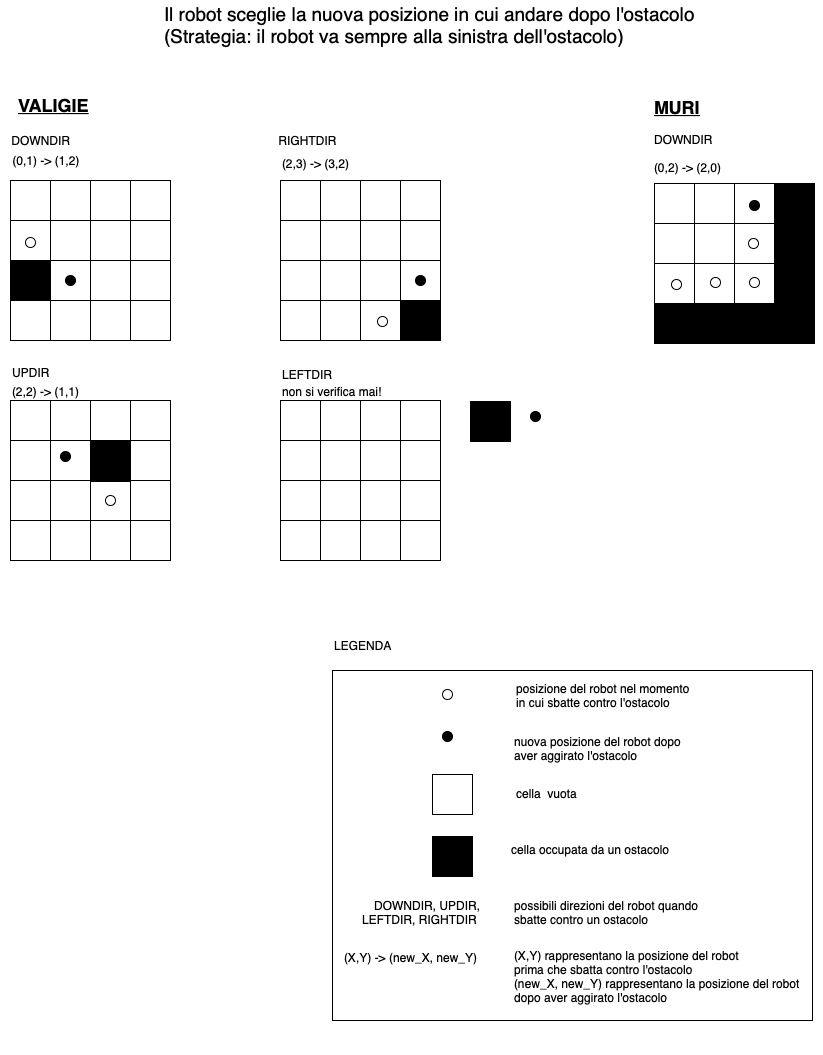
\includegraphics[scale=0.35]{img/sprint4/go_around_obstcl_strategy.png}
  \caption{Le varie casistiche che il robot potrebbe dover affrontare.}
  \label{fig:go_around_obstcl_strategy}
\end{figure}

Un'altra problematica riguarda la gestione della fase di "fine esplorazione" in quanto, una volta che il robot ha individuato i confini della stanza, potrebbero comunque essere rimaste delle celle inesplorate (riportate con uno 0 sulla mappa). Per risolvere questo problema è necessario che il robot le visiti una ad una.

\subsection{Model}

La logica di funzionamento di robotmind dovrà gestire la nuova tipologia di ostacolo (valigia). Partendo dal presupposto che il robot ispezionerà la stanza utilizzando la strategia della chiocciola (già implementata nello Sprint 2), la nuova logica applicativa del robot dovrà eseguire i seguenti passi:
\begin{enumerate}
\item  ogni volta che il robot sbatte contro un ostacolo, quest'ultimo viene segnato sulla mappa con una X (già implementata nello Sprint 2);
\item il robot elabora un nuovo piano per provare a raggiungere il goal prefissato, se il piano fallisce ne calcola uno nuovo;
\item quando il robot esaurisce i piani disponibili  per raggiungere il goal, significa che le coordinate del goal non rientrano nelle dimensioni della stanza e che entrambe i muri (muro lato sud e lato est) della stanza sono stati individuati;
\item in ultimo, il robot finisce di controllare le celle della stanza rimaste inesplorate (rappresentate con uno 0 sulla mappa). Per ogni cella ancora inesplorata, il robot verifica se la cella è vuota oppure occupata da un ostacolo. \end{enumerate}

Inoltre, la logica applicativa che riguarda la realizzazione effettiva del piano (doPlan) ed il suo successo o fallimento è stata estrapolata da robotmind ed incapsulata in un nuovo attore (planexecutor), che dato un goal (es. il robot deve raggiungere la posizione (2,2) nella stanza), verifichi se il goal può essere portato a termine e notifichi l'attore (robotmind) del suo successo o fallimento. Il codice di planexecutor è riportato nel Listing \ref{lst:planexecutor-ddr-sys-5}. Il Listing \ref{lst:robotmind-ddr-sys-5} contiene i messaggi sui quali starà in attesa robotmind a fronte della nuova spartizione dei compiti tra lui stesso e planexecutor.
Per quanto riguarda la gestione degli eventi del sonar si è ritenuto opportuno creare un QActor dedicato, denominato sonahandler. Questo QActor, ogni volta che cattura un evento sonarRobot, non invia alcun messaggio nel caso in cui il valore sia maggiore di una certa soglia, poichè significa che non è presente un ostacolo di fronte al robot, in caso contrario invia un messaggio all'attore onestepahead. 

\begin{lstlisting}[backgroundcolor=\color{white}, label={lst:planexecutor-ddr-sys-5}, caption={"Codice di planexecutor in ddrSystem5"}]

QActor planexecutor context robotMindCtx {
	["
		var Curmove     = \"\"  
		var Map = \"\"
		var Tback = 0
		var StepTime   = 330 
		//var StepTime   = 700 //fisico 

    "]
	State s0 initial {} 

	Transition t0  whenMsg doPlan  -> loadPlan
				 
	State loadPlan {
		printCurrentMessage
 		run itunibo.planner.moveUtils.doPlan( myself ) //moves stored in actor kb
	}
				 	
	Goto doPlan
	
 	State doPlan {	}
 	
	Transition t1 whenTime 50  -> doPlan1 		
 		          whenMsg stopCmd -> stopAppl
 		          
 	State stopAppl {
 		forward robotactuator -m robotCmd : robotCmd(h)
 		forward resourcemodel -m modelUpdate  : modelUpdate( robot, h ) 
 		solve(retractall( move(_)))
 	} 
 	
 	Goto s0
 	
 	State doPlan1{
 	
		["Map =  itunibo.planner.plannerUtil.getMapOneLine()"]
		forward resourcemodel -m modelUpdate  : modelUpdate( roomMap, $Map )
		run itunibo.planner.plannerUtil.showMap() 
		
		solve( retract( move(M) ) ) 	//consume a move
		ifSolved {  ["Curmove = getCurSol(\"M\").toString()"]  }
		else { ["Curmove=\"nomove\" "]  }

	}  
	
	Goto handlemove if "(Curmove != \"nomove\")" else planOk
	
	State planOk {
		forward robotactuator -m robotCmd : robotCmd(h)
		forward resourcemodel -m modelUpdate  : modelUpdate( robot, h ) 
		forward robotmind -m planOk : planOk 
	}
	
	Goto s0
	
	State handlemove {}
	
	Goto domove if "(Curmove != \"w\")" else attempttogoahead
	
	State domove {
		
		run itunibo.planner.moveUtils.doPlannedMove(myself, Curmove)
		forward robotactuator -m robotCmd : robotCmd($Curmove)
		delay 500 //fisico  
		forward robotactuator -m robotCmd : robotCmd(h)
	
		forward resourcemodel -m modelUpdate  : modelUpdate( robot, $Curmove ) 
	}
	
	Goto doPlan
	
	//roomboundaryplanning.qak
	State attempttogoahead {	
		forward resourcemodel -m modelUpdate  : modelUpdate( robot, w ) 
		run itunibo.planner.moveUtils.attemptTomoveAhead(myself, StepTime)
	}
	
	Transition t2   whenMsg stepOk   -> stepDone   
					whenMsg stepFail -> stepFailed
					 
 	State stepDone{  
 		forward resourcemodel -m modelUpdate  : modelUpdate( robot, h ) 
 		run itunibo.planner.moveUtils.doPlannedMove(myself, "w")	
 		
 	}
 	
 	Goto doPlan
 	
 	State stepFailed{
 		println("&&&  OBSTACLE FOUND") 
		["var TbackLong = 0L"]		 
 	  	
		//printCurrentMessage		        
 		onMsg( stepFail : stepFail(Obs, Time) ) { 
 			["Tback= (payloadArg(1).toLong().toString().toInt()*0.85 ).toInt()
			TbackLong = Tback.toLong()"]
 		}
  		
 		println(" backToCompensate stepTime=$Tback")
 		forward resourcemodel -m modelUpdate  : modelUpdate( robot, s ) 
 		forward robotactuator -m robotCmd : robotCmd(s)
		
		delayVar TbackLong
		
		forward robotactuator -m robotCmd : robotCmd(h)
		forward resourcemodel -m modelUpdate  : modelUpdate( robot, h ) 
		
		forward robotmind -m planFail : planFail 
		solve(retractall( move(_)))	
	}
	Goto s0	
}


\end{lstlisting}


\begin{lstlisting}[backgroundcolor=\color{white}, label={lst:robotmind-ddr-sys-5}, caption={"Codice di robotmind in ddrSystem5"}]



QActor robotmind context robotMindCtx { 

    ...

	State startExploration {
		println("&&&  exploration STARTED")
	
		run itunibo.planner.plannerUtil.setGoal(X,Y)
		forward planexecutor -m doPlan : doPlan($X,$Y)
	}
	
	Transition t1 ...
	              whenMsg planOk -> nextGoal
				  whenMsg planFail -> checkIfObstacle
				  
	State nextGoal {
		if "backHome" {
			["
			backHome = false
			X = 0
			Y = 0
			iterCounter++"]
		}
		else {
		["
			backHome = true
			X = iterCounter
			Y = iterCounter
		"]
		}
	}
	
	...
	
	State checkIfObstacle {
		println("---CheckIfObstacle---")
		run itunibo.planner.moveUtils.setObstacleOnCurrentDirection(myself)
		run itunibo.planner.plannerUtil.resetGoal(X,Y)
		run itunibo.planner.moveUtils.setObstacleOnCurrentDirection(myself)
		["plan = itunibo.planner.plannerUtil.doPlan()"]	
		
	}
	
    ...
}

\end{lstlisting}

L'architettura del sistema è riportata in \cref{fig:arch_logica_4}.

\begin{figure}[H]
  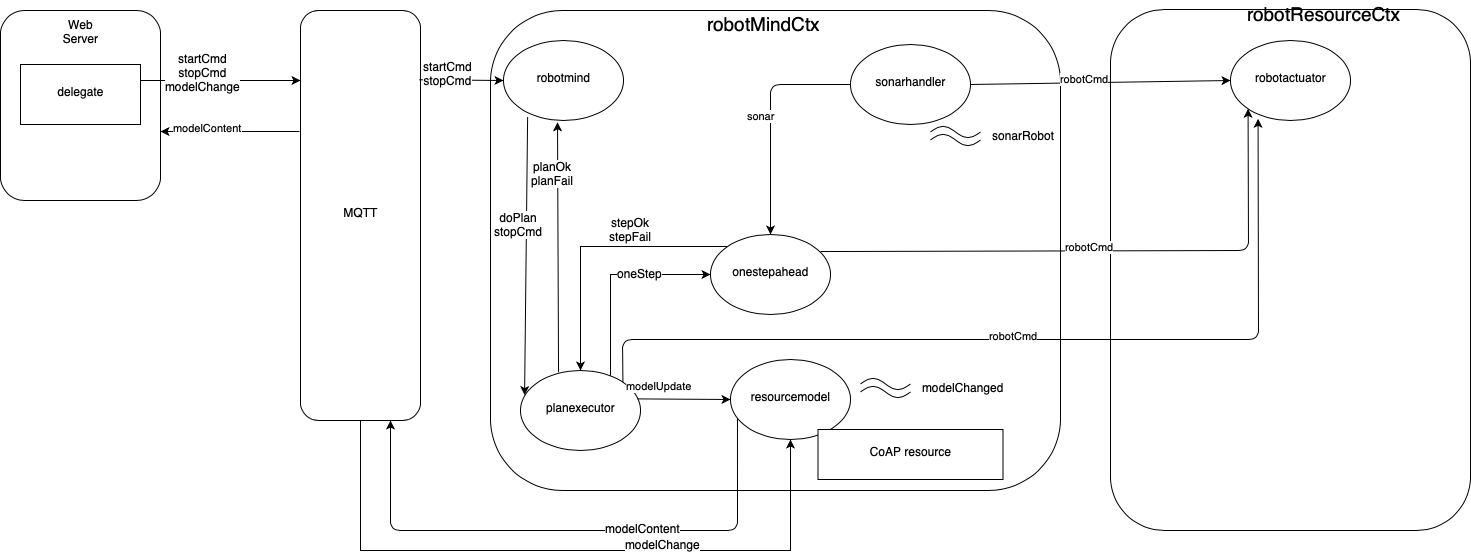
\includegraphics[width=\textwidth]{img/sprint4/arch_logica_4.png}
  \caption{L'architettura del sistema.}
  \label{fig:arch_logica_4}
\end{figure}


\subsection{Test plan}

Verificare il corretto funzionamento del sistema:

\begin{itemize}
\item durante la fase di esplorazione, quando il robot incontra un ostacolo, verificare che l'ostacolo venga segnalato correttamente sulla mappa;
\item una volta incontrato un ostacolo, verificare che il robot calcoli un nuovo piano per raggiungere il suo obiettivo;
\item verificare che, nel caso in cui l'obiettivo si trovi in corrispondenza di un ostacolo, il robot scelga il goal successivo senza bloccarsi;
\item verificare che, nel caso in cui un obbiettivo si trovi all'esterno dei confini il robot termini l'esplorazione;
\item verificare che, una volta determinati i confini della stanza, il robot esplori tutte le celle non ancora visitate;
\end{itemize}{}